\chapter{Literature Review}

\section{Introduction}

Bio-inspired robots have fascinated humans since the Greek mathematician, Archytas of Tarentum, built the first true mechanical robot, where a robot is some device performing an automated mechanical task. His mechanical steam powered bird was just the start.\cite{Isom2005}   

Would be engineers take their inspiration from popular culture with The Iron Giant and B.E.N. fresh in mind. The Rising Sun included robots developed by Marc Raibert, founder of the CMU (now MIT) Leg Laboratory, who pioneered self-balancing dynamic control of hopping robots. 

\begin{figure}
\centering
\subfloat[][The Iron Giant (1999).]{
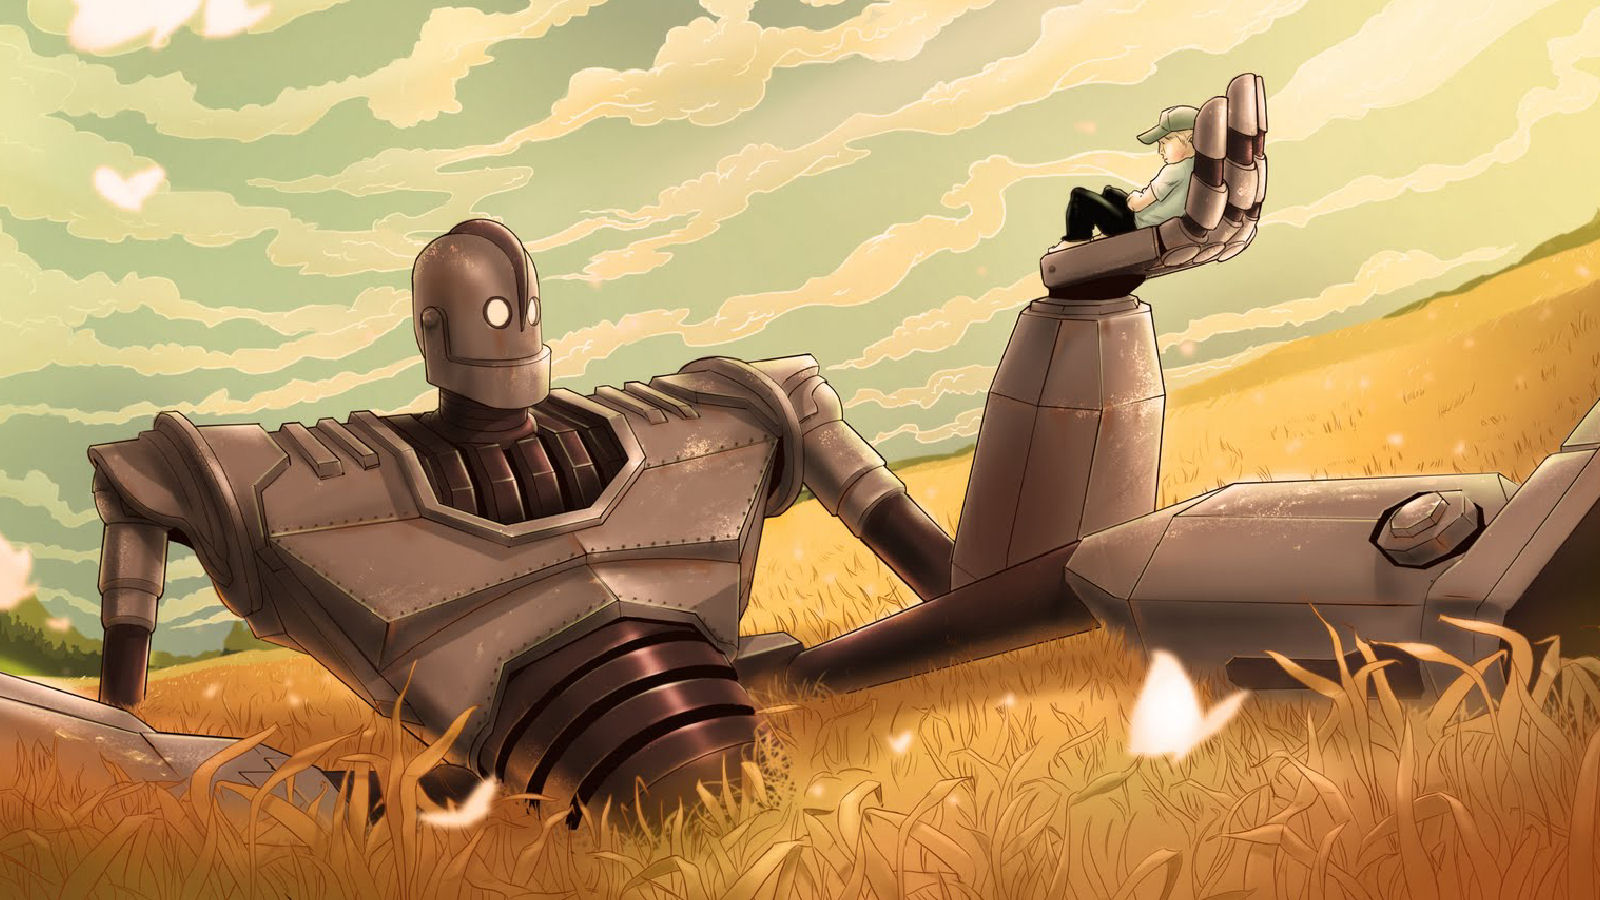
\includegraphics[width=0.6\textwidth]{images/literature/the-iron-giant-1999.jpg} 
\label{fig:the-iron-giant-1999}
}

\subfloat[][Rising Sun (1993).]{
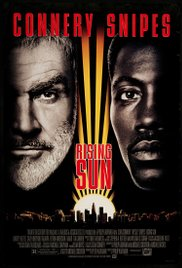
\includegraphics[width=0.3\textwidth]{images/literature/rising-sun.jpg} 
\label{fig:rising-sun}
}
\subfloat[][Treasure Planet (2002).]{
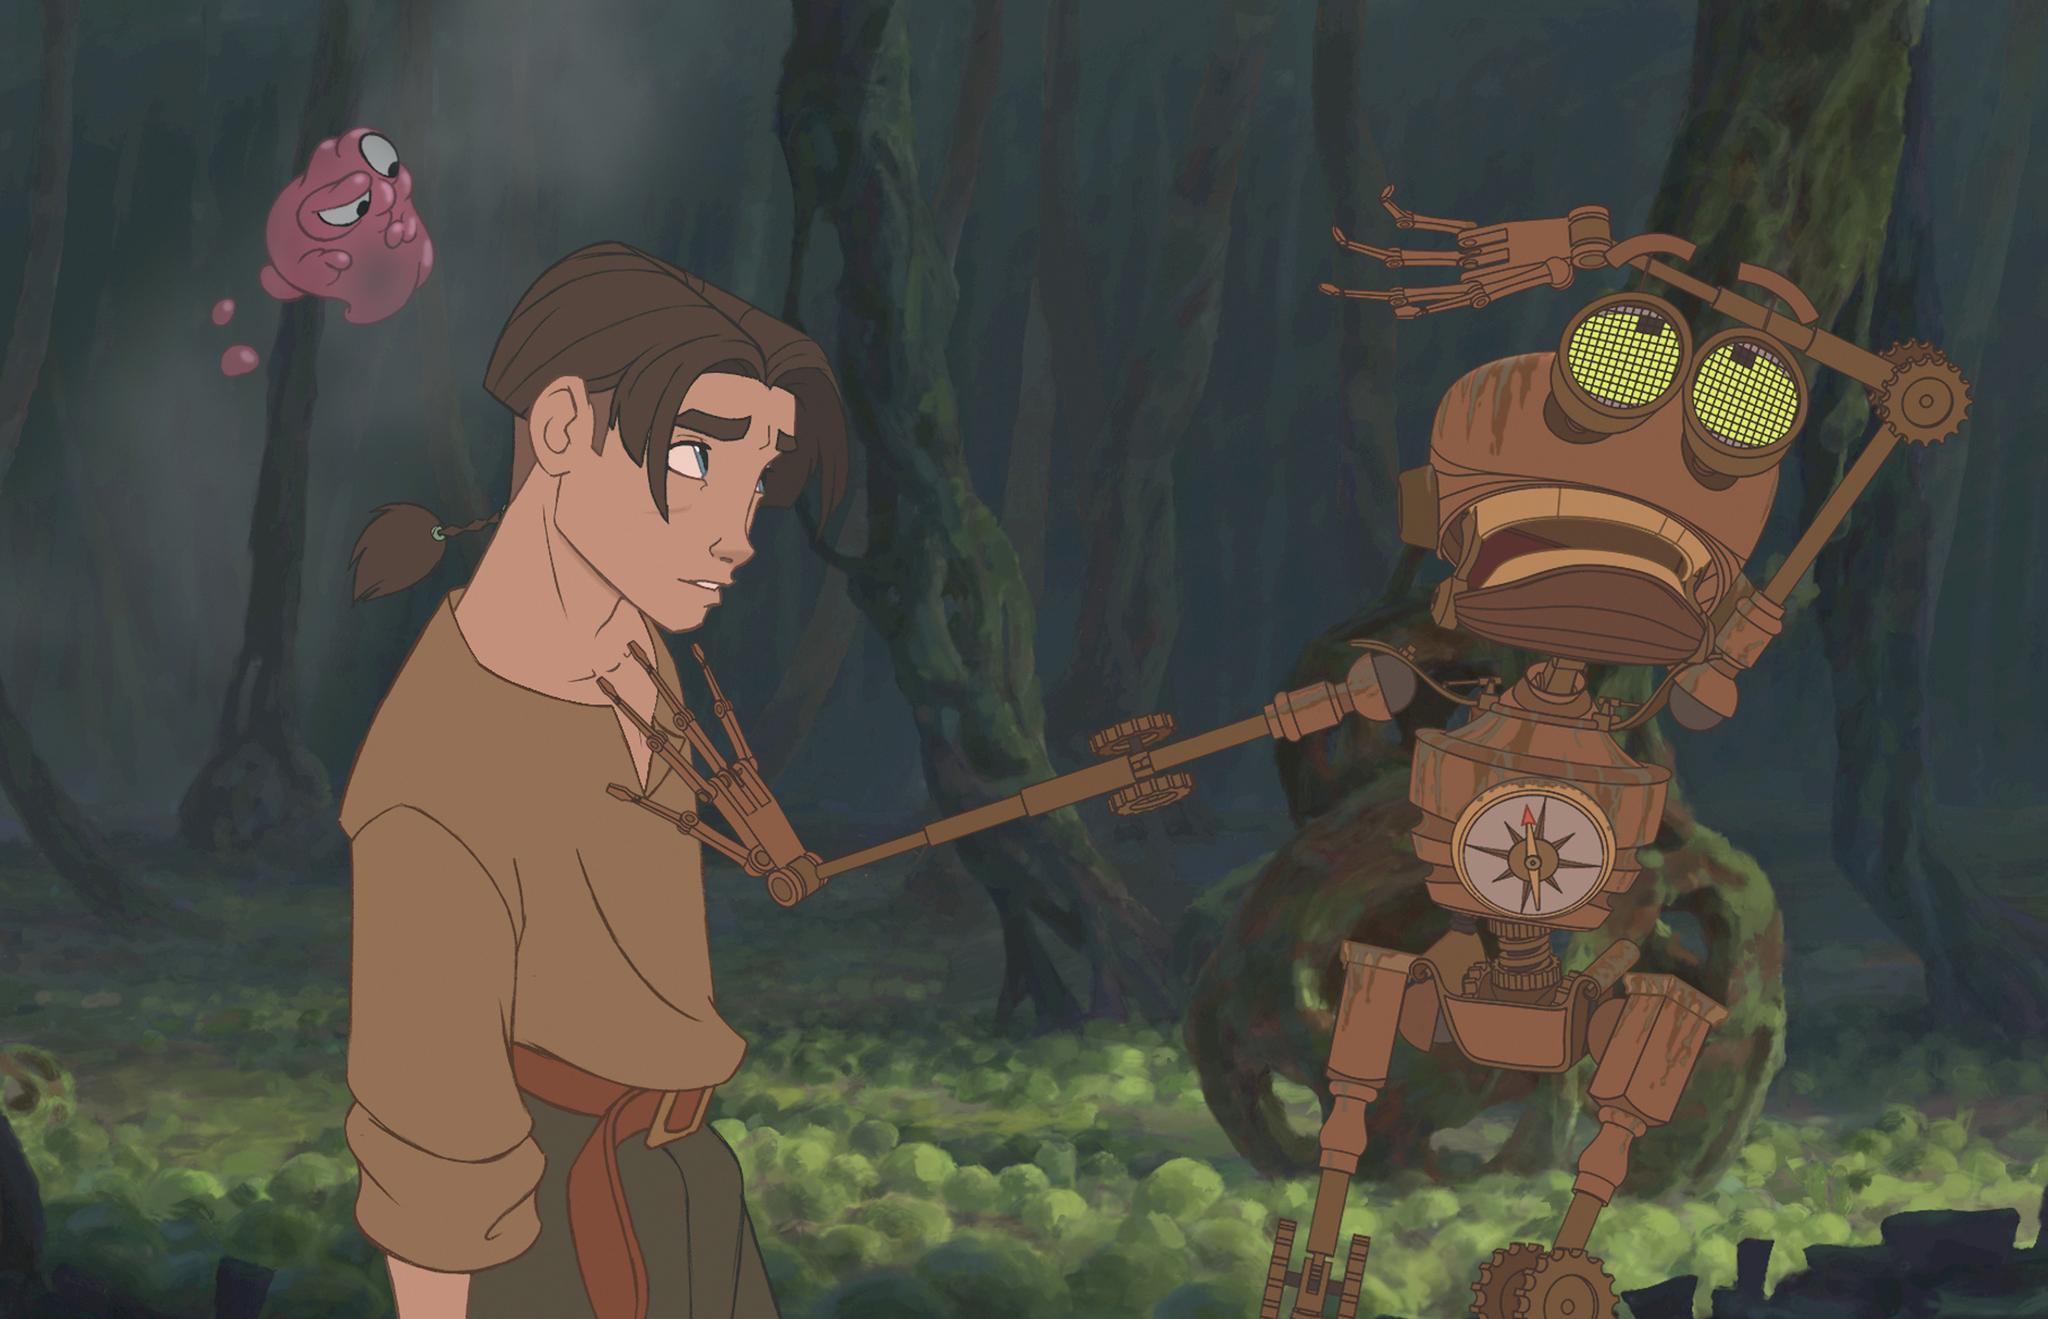
\includegraphics[width=0.3\textwidth]{images/literature/BEN-treasure-island-2002.jpg} 
\label{fig:BEN-treasure-island-2002}
}
\caption{Humanoid robots in popular culture.}
\end{figure}

\section{State of the Art}

\subsection{Monoped Robots}

\begin{figure}
\centering
\subfloat[][Planar One-Leg Hopper - MIT Leg Laboratory (1980-1982).]{
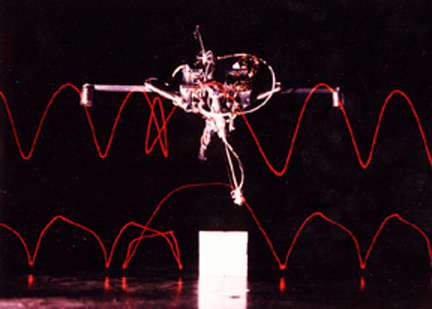
\includegraphics[width=0.3\textwidth]{images/literature/planar-one-leg-hopper.jpeg} 
\label{fig:planar-one-leg-hopper}
}
~
\subfloat[][3D One-Leg Hopper - MIT Leg Laboratory (1983-1984).]{
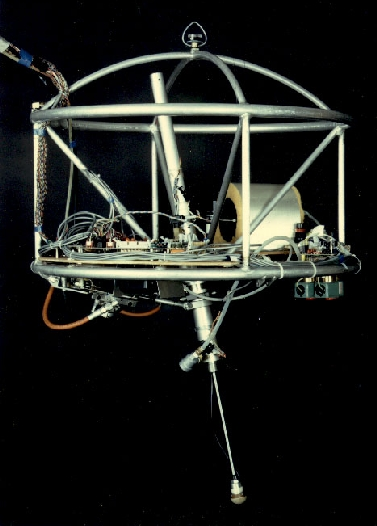
\includegraphics[width=0.3\textwidth]{images/literature/3D-one-leg-hopper.jpeg} 
\label{fig:3D-one-leg-hopper}
}
\caption{Monoped robots.}
\label{monoped-robots}
\end{figure}


\subsection{Biped Robots}

\begin{figure}
\centering
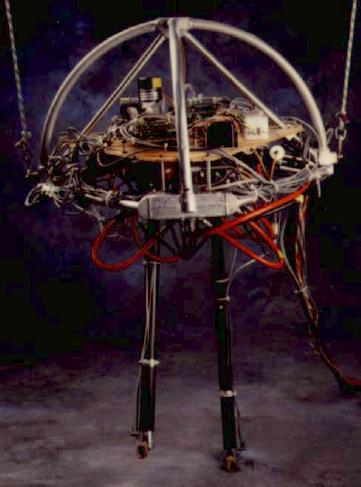
\includegraphics[width=0.3\textwidth]{images/literature/3D-biped.jpeg} 
\caption{3D Biped - MIT Leg Laboratory (1989-1995).}
\label{fig:3D-biped}
\end{figure}


\subsection{Quadruped Robots}

\begin{figure}
\centering
\subfloat[][Quadruped - MIT Leg Laboratory (1984-1987).]{
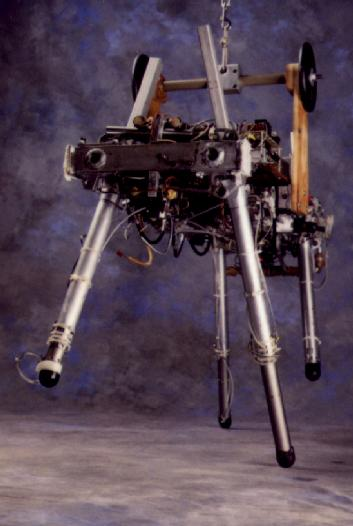
\includegraphics[width=0.3\textwidth]{images/literature/quadruped.jpeg} 
\label{fig:quadruped}
}
~
\subfloat[][GOAT 3-DOF Leg Topology - (Kalouche, 2016).]{
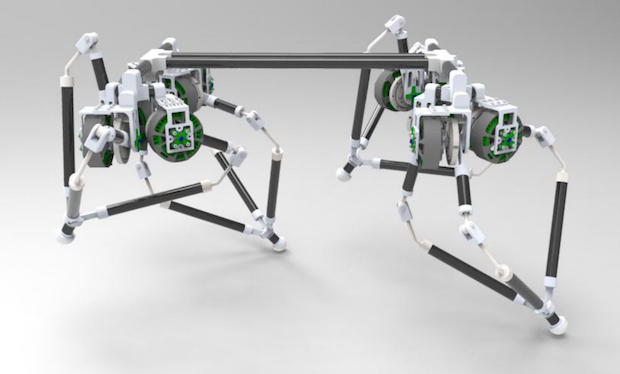
\includegraphics[width=0.3\textwidth]{images/literature/goat-leg.jpeg} 
\label{fig:goat-leg}
}
\caption{Quadruped robots.}
\label{Quadruped-robots}
\end{figure}


\subsection{Bio-inspired Legged Robotics}

\begin{figure}
\centering
\subfloat[][Uniroo - MIT Leg Laboratory (1991-1993).]{
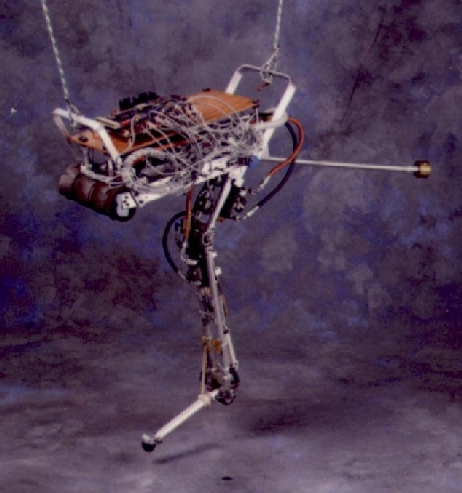
\includegraphics[width=0.3\textwidth]{images/literature/uniroo-bioinspired.jpeg} 
\label{fig:uniroo-bioinspired}
}
~
\subfloat[][Spring Flamingo - MIT Leg Laboratory (1996-2000).]{
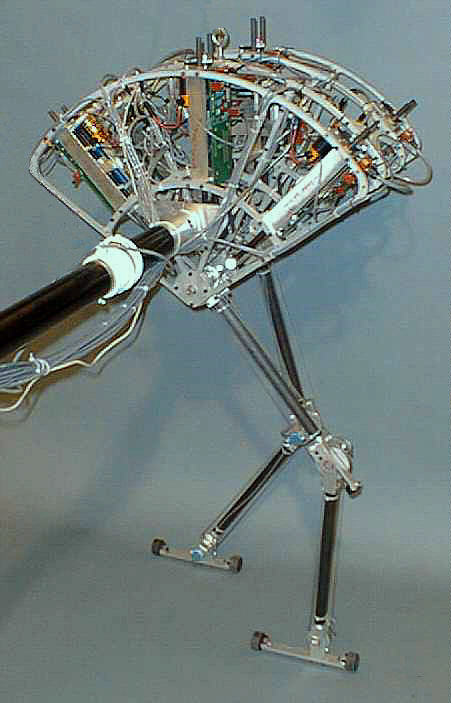
\includegraphics[width=0.3\textwidth]{images/literature/spring-flamingo.jpg} 
\label{fig:spring-flamingo}
}
\caption{Bio-inspired legged robots.}
\label{bioinspired-legged-robots}
\end{figure}

\subsection{Humanoid Robots}

\begin{figure}
\centering
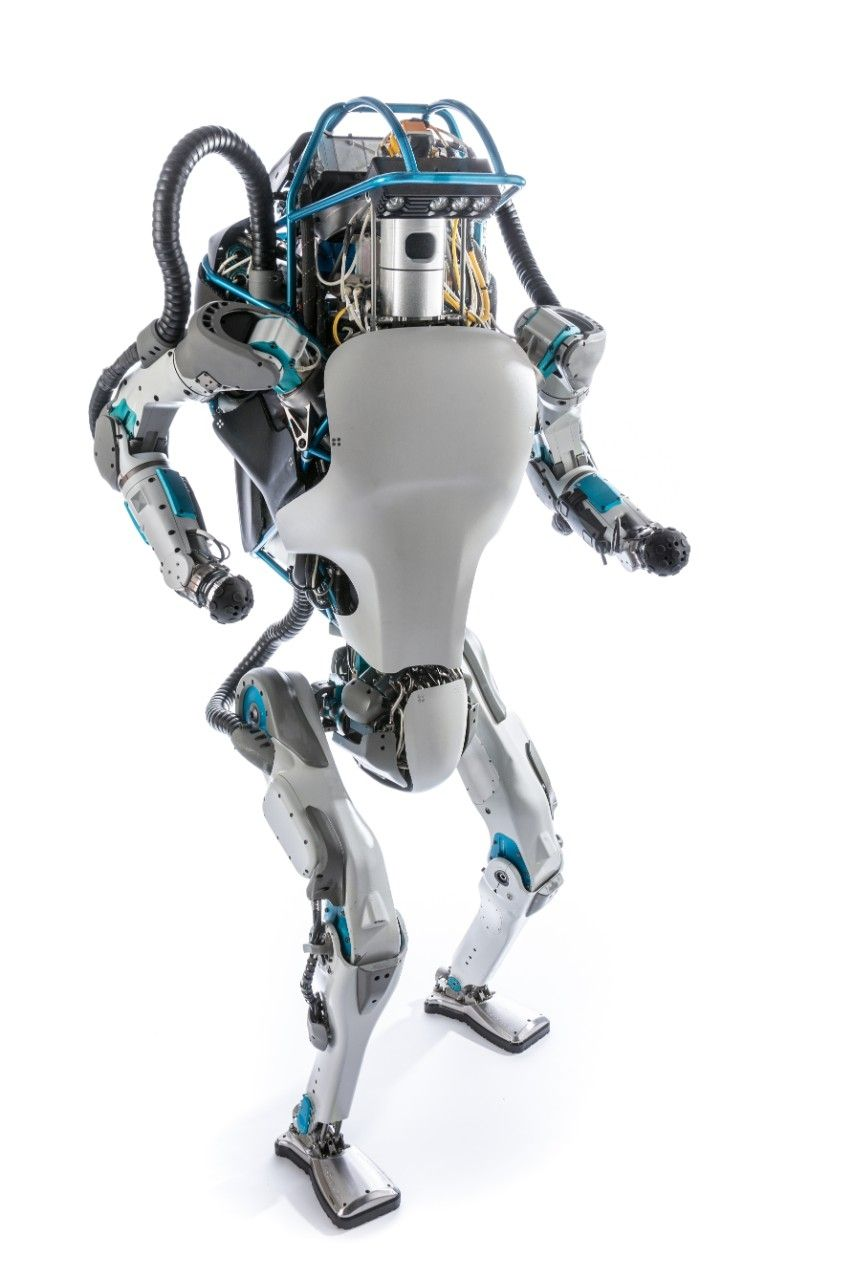
\includegraphics[width=0.3\textwidth]{images/literature/atlas-humanoid.jpg} 
\caption{Atlas Humanoid Robot - Boston Dynamics (2013).}
\label{fig:Atlas Humanoid Robot}
\end{figure}

\subsection{Closed Kinematic Chain Leg}

\begin{figure}
\centering
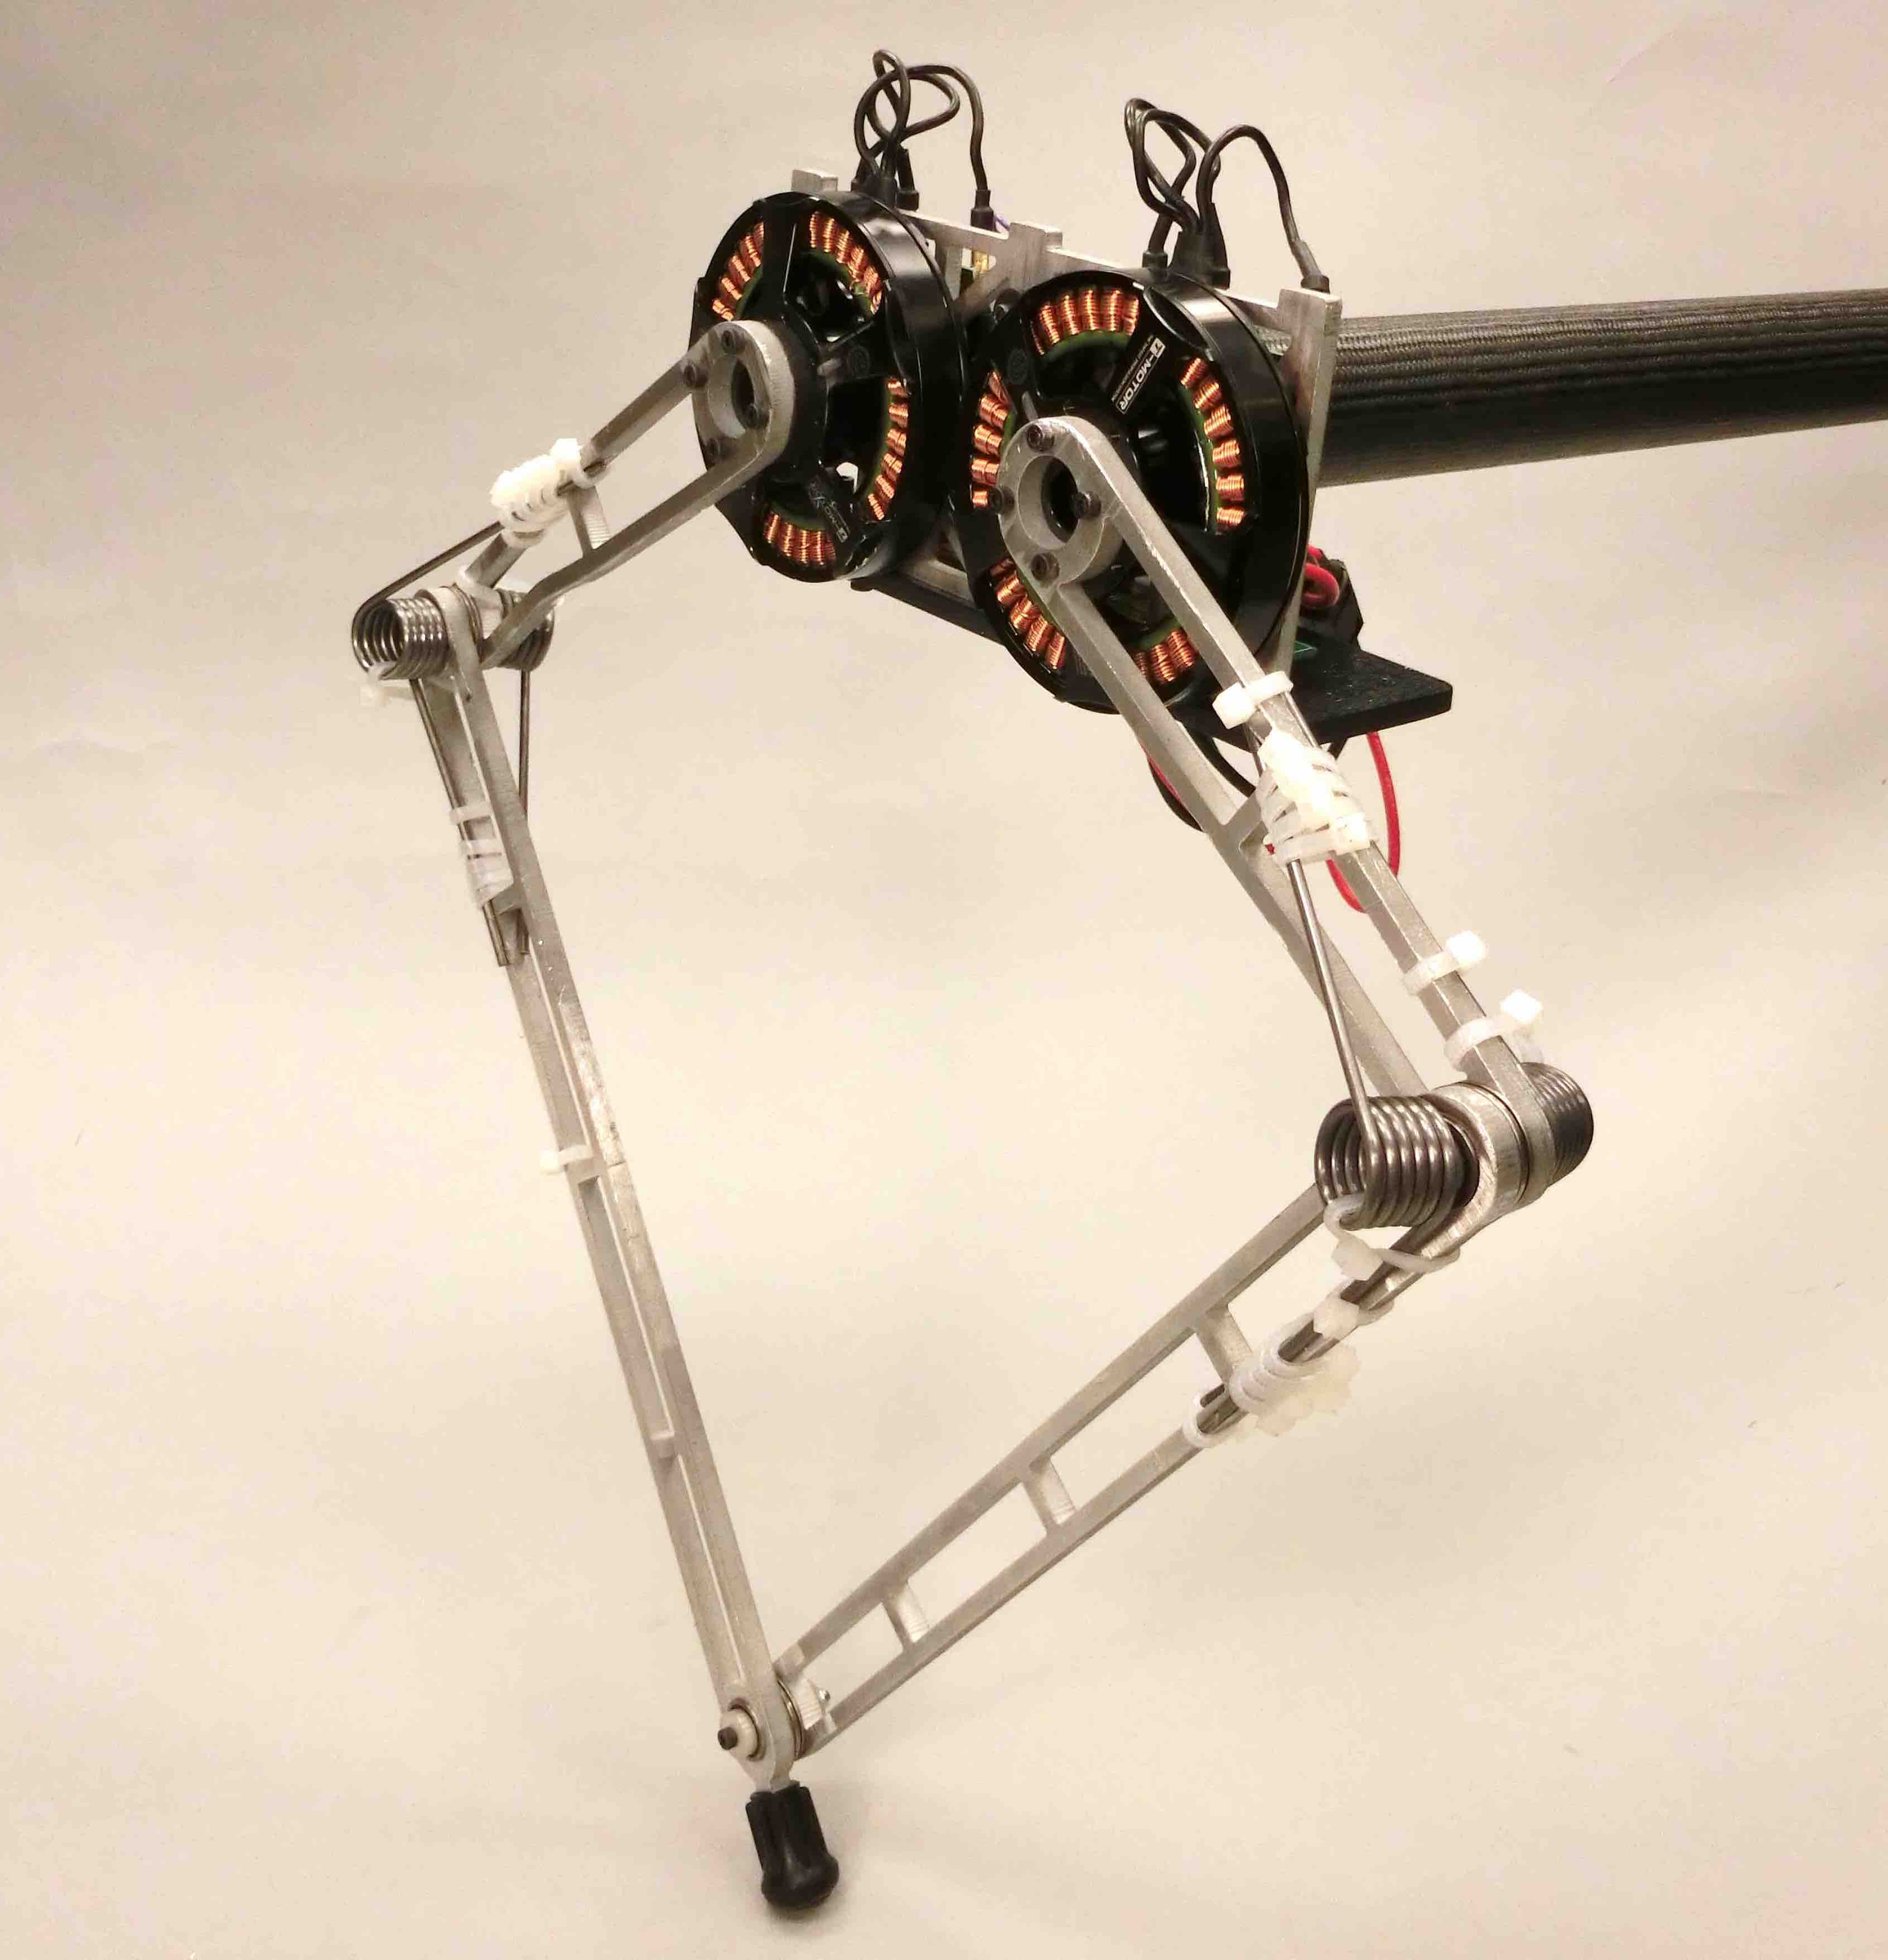
\includegraphics[width=0.5\textwidth]{images/literature/pen-state-scissor.jpg} 
\caption{Closed Kinematic Chain Leg using Raibert's Scissor Algorithm (Duperret, Koditschek, 2016).\cite{Duperret}}
\label{fig:pen-state-scissor}
\end{figure}

\section{Legged Locomotion in Nature}

\section{Raibert Control}

\begin{figure}
\centering
\subfloat[][Legged Robots That Balance - Marc H. Raibert (1986).]{
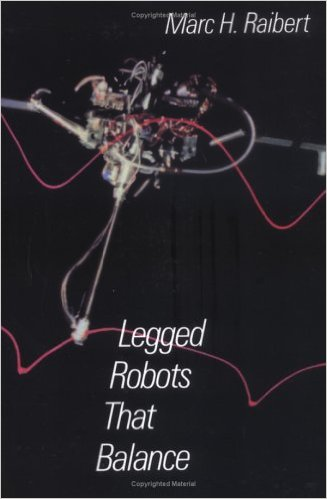
\includegraphics[width=0.3\textwidth]{images/literature/legged-robots-that-balance.jpg} 
\label{fig:legged-robots-that-balance}
}
~
\subfloat[][Raibert control state machine.]{
\includegraphics[clip, trim=7cm 19cm 7cm 2cm, page = 25, width=0.5\textwidth]{"pdfs/Raibert et al - 1989 - Dynamically Stable Legged Locomotion (September 1985-Septembers1989)"}
\label{fig:Raibert control state machine}
}
\caption{Legged Robots That Balance cover page and exert.\cite{Raibert1989}}
\end{figure}

\subsection{Raibert's Scissor Algorithm}

\subsection{Phases of Motion}

\section{Applications in Industry}
\subsection{Soft-robotics}
Factories safe human robot interaction
Handling of compliant products (farming, manufacturing)


\begin{figure}
\centering
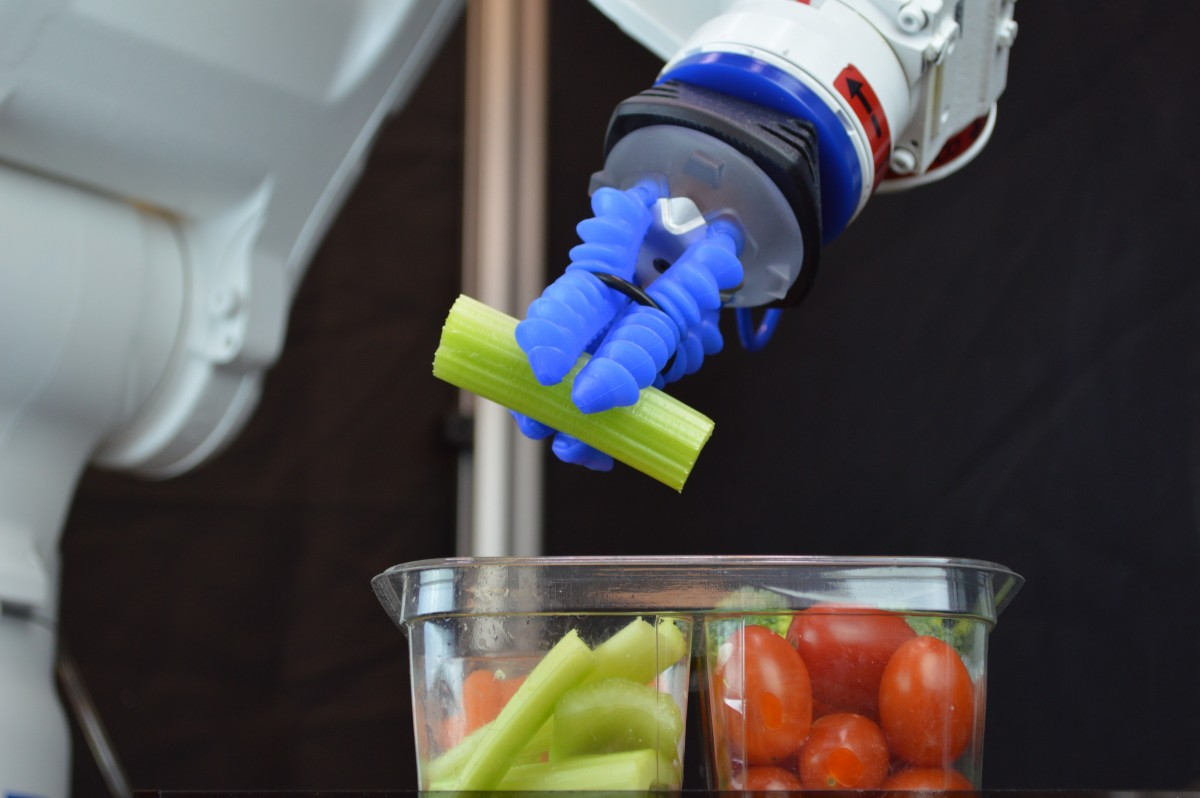
\includegraphics[width=0.6\textwidth]{images/literature/SoftRobotCelery} 
\caption{Compliant soft robotic handling (Forbes, 2016).}
\label{fig:Compliant soft robotic handling}
\end{figure}
\cite{Knapp}

\subsection{Bose Active Suspension}

\begin{figure}
\centering
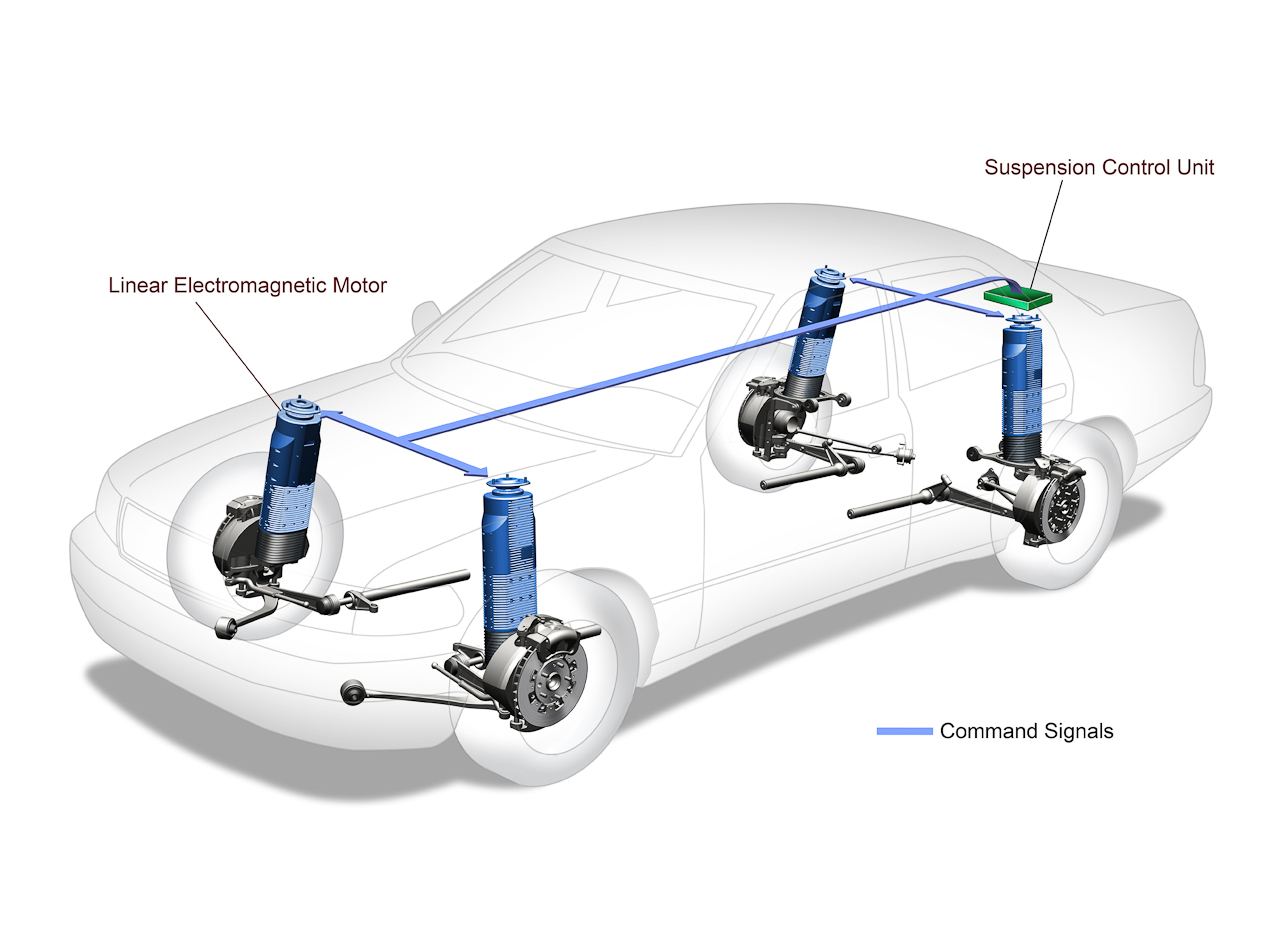
\includegraphics[width=0.6\textwidth]{images/literature/Bose-suspension-system.jpg} 
\caption{Bose Active Suspension (Bose Corporation, 1980s)\cite{Bose}.}
\label{fig:Bose Active Suspension}
\end{figure}

\subsection{Dynamic Stability vs Static Stability}
\subsection{Phases of Motion}
\subsection{Leg Stance Control}
\section{Force Control}
